\documentclass[a4paper,12pt,reqno]{amsart}
\usepackage{macros_M43}

\begin{document}

% ===================================================================
\hautdepage{Fiche 4: Vecteurs aléatoires discrets}
% ===================================================================


%-----------------------------------
\begin{exo}

  Les variables aléatoires $X$ et $Y$ sont telles que:
    $$
      \begin{array}{ccc}
                                   & P(X=0 \text{ et } Y=1)=1/5 & P(X=0 \text{ et } Y=2)=1/5 \\
        P(X=1 \text{ et } Y=0)=1/5 & P(X=1 \text{ et } Y=1)=1/5 & P(X=1 \text{ et } Y=2)=1/5
      \end{array}
    $$
  \begin{enumerate}
    \item Déterminer la loi de $X$.
    \item Déterminer la loi de $Y$.
    \item Les variables aléatoires $X$ et $Y$ sont-elles indépendantes?
    \item Trouver la loi de $Z = X-Y$.
  \end{enumerate}

\end{exo}

%-----------------------------------
\begin{exo}

  La loi du couple $(U,V)$ est de la forme:
    $$
      P(U=j,V=k)=C\frac{k}{j!(60-j)!} \quad\text{ pour } k\in\{1,2,\ldots,59\} \text{ et } j\in\{0,1,\ldots,60\}
    $$
  \begin{enumerate}
    \item Pour connaître vraiment la loi du couple, il faut connaître la constante réelle $C$ dont on ne nous a pas donné la valeur. Calculer $C$.
    \item Calculer la loi de $U$ (et donner son nom si elle en a un).
    \item Calculer la loi de $V$ (et donner son nom si elle en a un).
    \item $U$ et $V$ sont-elles indépendantes?
  \end{enumerate}

\end{exo}

%-----------------------------------
\begin{exo}

  On suppose que le couple de variables aléatoires discrètes $(X,Y)$ a une loi donnée par:
    $$
      \forall (i,j)\in\N^{2},\quad P(X=i, Y=j)=\frac{\alpha}{(1+i+j)!},
    $$
  où $\alpha$ est une constante strictement positive qui sera précisée ultérieurement.
  \begin{enumerate}
    \item Expliquer sans  calcul pourquoi les marginales $X$ et $Y$ ont même loi.
    \item On pose $S=X+Y$. Montrer que:
      $$
        \forall k\in\N,\quad P(S=k)=\frac{\alpha}{k!}.
      $$
    \item En déduire la valeur de $\alpha$ et reconnaître la loi de $S$.
    \item Calculer $P(X=0)$. Les variables aléatoires $X$ et $Y$ sont-elles indépendantes?
    \item Calculer $P(X=Y)$ et en déduire sans calcul $P(X>Y)$.
  \end{enumerate}

\end{exo}

%-----------------------------------
\begin{exo}

  Soient $T$ et $U$  deux variables aléatoires indépendantes de loi géométriques de paramètres $\alpha$ et $\beta$ (avec $\alpha$ et $\beta$ fixés dans $]0,1[$).
  \begin{enumerate}
    \item Calculer la loi de leur somme $T+U$, dans le cas où $\alpha\neq\beta$, puis dans le cas où $\alpha=\beta$.
    \item En déduire que quand $\alpha=\beta$, $T+U$ est la loi du second succès dans une suite d'épreuves indépendantes où la probabilité de succès vaut $\alpha$.
    \item Dans le cas $\alpha=\beta$, calculer $P(T \neq U)$.
  \end{enumerate}

\end{exo}

%-----------------------------------
\begin{exo}

  Lors d'un congrès à Grenoble, $n$ chercheurs se répartissent de façon aléatoire et indépendamment les uns des autres dans les $r > 1$ hôtels, $H_1,\ldots,H_r$, de la ville. On désigne par $p_i \in\, ]0,1[$ la probabilité qu'un chercheur aille dans l'hôtel $H_i$, de sorte que $\sum_{i=1}^rp_i=1$ pour $i\in\{1,\ldots,r\}$, et par $X_i$ le nombre de personnes qui vont dans l'hôtel $H_i$.
  \begin{enumerate}
    \item Soit $i\in\{1,\ldots,r\}$. Quelle est la loi de $X_i$ ?
    \item Déterminer  $P(X_1=n_1,\ldots,X_r=n_r)$ pour tout $r$-uplets $(n_1,\ldots,n_r)$ tel que $n_1+\ldots +n_n=n$.
    \item Les variables $X_i$ sont-elles deux à deux indépendantes ?
  \end{enumerate}

\end{exo}

%-----------------------------------
\begin{exo}

  Pour les besoins médicaux (en particulier les transfusions), on classe le sang humain en quatre groupes: groupe O, groupe A, groupe B et groupe AB. Mais le sang présente aussi un « facteur rhésus », qui peut être positif ou négatif. Il y a donc huit\footnote{Il y a en réalité beaucoup plus de catégories, basées sur une trentaine de caractéristiques du sang. Mais les deux caractéristiques ci-dessus (ABO et rhésus) sont les plus importantes pour assurer la compatibilité des transfusions. Et ces deux caractéristiques ne déterminent que huit catégories.} catégories de sang (O positif, O négatif, A positif, A négatif, etc).

  En France, une personne choisie au hasard a $43\%$ de chances d'être du groupe O, $45\%$ de chances d'être du groupe A, $9\%$ de chances d'être du groupe B, et $3\%$ de chances d'être du groupe AB. Parmi les personnes du groupe O, $14\%$ sont de rhésus négatif. La proportion de rhésus négatif est de $13\%$ parmi les personnes du groupe A. Elle est de $22\%$ parmi les gens de groupe sanguin B, et de $33\%$ parmi les personnes du groupe AB.
  \begin{enumerate}
    \item Quelle est la probabilité qu'une personne prise au hasard soit de rhésus positif?
    \item Si l'on sait qu'une personne est de rhésus négatif, quelle est la probabilité qu'elle soit du groupe AB?
    \item Dans un groupe de TD de 24 étudiants, on note $N_O$, $N_A$, $N_B$ et $N_{AB}$ les nombres respectifs d'étudiants ayant le groupe sanguin O, A, B et AB. Quelle est la loi du vecteur aléatoire  $(N_O,N_A,N_B,N_{AB})$? Indiquer aussi les quatre lois des variables aléatoires $N_O$, $N_A$, $N_B$ et $N_{AB}$.
    \item Quelle est la loi du couple aléatoire $(N_O+N_A,N_B+N_{AB})$?
  \end{enumerate}
\end{exo}

%-----------------------------------
\begin{exo}

  \begin{minipage}{.77\linewidth}
  Dans tout cet exercice, le vecteur aléatoire discret $(X,Y)$ a pour support $S$ l'ensemble des six points représentés sur la figure ci-contre. La loi de $(X,Y)$ est donc donnée par les $P\big((X,Y)=(i,j)\big)$, pour $(i,j)\in S$.
  \end{minipage}%
  \begin{minipage}{.21\linewidth}
    \hfill
    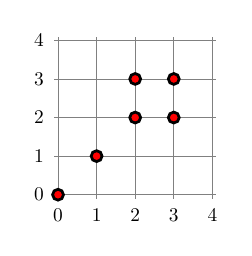
\begin{tikzpicture}[outer sep=4pt,scale=.49]
      \draw[help lines] (-.1,-.1) grid (4.1,4.1);
      \foreach ~ in {0,...,4}{
        \node[below,scale=.7] at (~,0) {~};
        \node[left,scale=.7] at (0,~) {~};
      }
      \foreach \x/\y in {0/0,1/1,2/2,2/3,3/2,3/3}
        \filldraw[fill=red, line width=1pt] (\x,\y) circle(4pt);
    \end{tikzpicture}
  \end{minipage}
    \begin{enumerate}
      \item Quelles probabilités faut-il attribuer aux différents points de $S$ pour satisfaire simultanément aux deux conditions suivantes~:
      \begin{enumerate}
        \item\label{conda} les points de $\iintv{2,3}^2$ ont tous même probabilité,
        \item\label{condb} $X$ et $Y$ suivent la loi uniforme sur $\iintv{0,3}$ ?
      \end{enumerate}
      \item Lorsque $(X,Y)$ suit la loi déterminée à la question précédente, $X$ et $Y$ sont-elles indépendantes ? On peut répondre sans calcul.
      \item Montrer qu'il existe une infinité de lois de $(X,Y)$ avec support $S$ telles que \ref{condb} soit vérifiée et $X$ et $Y$ non indépendantes.
    \end{enumerate}

\end{exo}


\end{document}

